\documentclass[conference]{IEEEtran}
\usepackage{graphicx}
\usepackage{algorithm}
\usepackage{algorithmicx}
\usepackage{algpseudocode}
\usepackage[dvipsnames]{xcolor}
\usepackage{amsmath}

\algblock{Input}{EndInput}
\algnotext{EndInput}
\algblock{Output}{EndOutput}
\algnotext{EndOutput}
\newcommand{\Desc}[2]{\State \makebox[5em][l]{#1}#2}

\newenvironment{conditions}
  {\par\vspace{\abovedisplayskip}\noindent\begin{tabular}{>{$}l<{$} @{${}={}$} l}}
  {\end{tabular}\par\vspace{\belowdisplayskip}}

\begin{document}
\title{I/O simulation extension for SimGrid framework}
\author{Hoang-Dung Do}
\maketitle

	\begin{abstract}
		\begin{itemize}
			\item The I/O bottleneck in HPC and the need of experiments.
			\item HPC experiment frameworks and advantages of SimGrid.
			\item The missing of the ability to simulate page cache, the goal of this paper.
			\item Principle of the simulator, experiment scenarios and comparisons.
			\item Brief discussion on results and future work.
		\end{itemize}
	\end{abstract}

	\section{Introduction}
		\begin{itemize}
			\item HPC, the bottleneck in I/O and the demand of HPC experiments. 
			\item Difficulties in conducting high performance computing experiments and the need of simulation frameworks.
			\item Existing experiment methods, simulators, simulation frameworks. The advantages of SimGrid compared to others \cite{casanova2008, lebre2015}. The missing of the ability to simulate page cache in SimGrid \cite{lebre2015}.
			\item The objective of the paper: Add capability to simulate I/O with page cache in SimGrid.
		\end{itemize}
	\section{Related Work}			
		
		\subsection{Page cache}
			\begin{itemize}
				\item What is page cache? How it works \cite{linuxdev3rd2010}. Effects and importance of page cache.
				\item Introduce some existing strategies with some highlighted pros and cons.
				\item Current implementation in Linux and some reasons why it is chosen to be implemented (implementation complexity, effectiveness, overhead, etc) \cite{linuxdev3rd2010}
			\end{itemize}									

		\subsection{Simulators}
			\begin{itemize}
				\item Discuss some existing methods, simulation frameworks to conduct HPC experiments. Compare pros and cons (accuracy, simulation time, usability) of some simulators (SimGrid, GridSim).
				\item Related development: RAM energy consumption \cite{gill2019} \cite{ouarnoughi2017} 
				\item Discuss the pros of SimGrid and the reasons why we chose it to extend. (Section 2.2.2 in \cite{casanova2014})
			\end{itemize}
			
	\section{Method}
		In this section, we discuss our approach to model page cache and the cache eviction strategy implemented in Linux. We also detail the design the simulators in order to generalize page cache as well as the implementation in Python and SimGrid framework. Finally, we describe some experimental scenarios to compare the results of Python simulator, baseline SimGrid simulator and the results from the real pipelines.
		\subsection{Principle of the simulator}
	
			When modeling the I/O time, we consider the key factors of the I/O mechanism having the biggest impacts on data read/write. The first factor taken into account is the use of the page cache in Linux kernel. In addition, the kernel controls I/O activities based on the status of the memory including the information about the cache size, the amount of available memory and dirty data. As these are managed and changed with the flushing and cache eviction mechanisms implemented in the kernel, data flushing and cache eviction must be generalized. The simulator should also make system parameters such as dirty{\_}ratio and dirty{\_}background{\_}ratio configurable since they can vary in different systems.
			
			The idea of our simulator is to generalize the memory, the page cache, the LRU lists, storage device and mimic the cache eviction algorithm implemented in the kernel. As for storage devices, we can leverage the storage model with disk capacity and disk bandwidth implemented in SimGrid \cite{lebre2015}. Because memory capacity and bandwidth are fixed, they can be kept as constants, while the amount of cache is dynamically allocated based on the amount of available memory. The simulator also keeps track of the LRU lists as in the kernel since they are the key component in cache eviction algorithm. However, maintaining and handling pages, which are in packet level, are non-trivial when they require significant implementation overhead and hinder the performance of the simulator. To simplify cache eviction while preserving accuracy, in our approach, we consider a sequence of continuously accessed pages of a file as a single unit, a block of data. The information of a single page in a sequence can be used as the representative for other pages in a sequence since they have the same properties including file name, last access, the page is dirty or not. Hence, instead of dealing with individual pages, we consider a sequence of continuously accessed pages as a block of data. A data block keeps the information about file name, block size, last access and a dirty flag describing whether the data is dirty or not. Since a block represents a set of pages in real systems, it can be split if some data needs to be moved between the LRU lists or evicted from cache, but blocks can not be merged as we want to preserve this level of granularity to maintain the accuracy. Having these components, we can generalize I/O activities in our simulator. When the kernel reads and writes data, it simply reads/writes data from/to disk or cache with predefined disk bandwidth or memory bandwidth. In flushing and periodical flushing, the kernel traverses through the inactive and active lists to reduce the amount of dirty data, while cache eviction algorithm deletes blocks from the inactive list. The LRU lists are updated after every I/O action.
			
			We create an extra layer with kernel-like functionalities between user application and SimGrid as is shown in Figure~\ref{fig:interaction}. Our new layer including two main additional classes, the \textbf{\textit{IOController}} class, which mimics the kernel I/O controlling logic, and the \textbf{\textit{MemoryManager}} class, which stores all necessary information about memory including capacity, the amount of cache, amount of memory used by applications, and manages LRU lists. Because every node has its own memory, storage devices and system configurations, there is one IOController object and one MemoryManager object created for each node. The IOController class keeps system parameters (dirty{\_}ratio, dirty{\_}background{\_}ratio), implements necessary I/O control functionalities such as read, write, flushing, and cache evicting. With these new components, instead of sending read/write requests directly to storage devices as in simulators with the current SimGrid version, user simulated applications send requests to an IOController of the node where requested data is stored. Based on the memory status in MemoryManager, the IOController orchestrates cache read/write, disk read/write, flushing and cache eviction to fulfill application requests. The time for each action is estimated and the total time of a request is returned to user applications.
				
			\begin{figure}
   				\centering
   				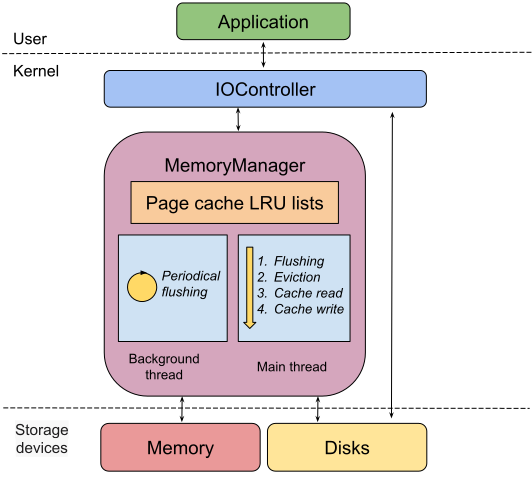
\includegraphics[width=0.85\columnwidth]{figures/interaction.pdf}
   				\caption{The additional layer between user application layer and original SimGrid API}\label{fig:interaction}
			\end{figure}
			
			\begin{algorithm}\caption{Read}\label{alg:read}
				\small
				\begin{algorithmic}[1]
					\Input
        				\Desc{$file\_name$}{file name}
			        	\Desc{$run\_time$}{current simulated run time}
   					\EndInput
					\State $mem\_required \gets max(0, 2* $file size$-cached\_data -$ available memory)
					\State $mem\_avail \gets max(0, 2 *$ file size$ - cached\_data -$ dirty data)
					\If {$mem\_required > mem\_avail$}
    					\State $run\_time \gets run\_time + $  flushing $(mem\_required - mem\_avail)	$
					\EndIf
										
					\State $free\_mem\_required \gets max(0, 2 *$ file size $- cached\_data -$ free memory)
					\If {$free\_mem\_required > 0$}
						\State evict from cache $(free\_mem\_required)$
					\EndIf
						
					\If {$cached\_data > 0$}
    					\State update cached blocks in LRU lists with the last access
						\If {all file data is cached}
    						\State $cache\_read\_time \gets cached\_data /$ memory read bandwidth
    						\State periodically flush $($flushing time $= cache\_read\_time)$
    						
							\Return $run\_time \gets run\_time + cache\_read\_time$
						\EndIf
					\EndIf

					\If {$cached\_data <$ file size}
						\If {dirty amount $> 0$} 
							\State $run\_time \gets run\_time +$ dirty amount flushing time
						\EndIf
						\State read from disk (amount from disk, $file\_name$), add accessed data to inactive list
    					\State $run\_time \gets run\_time +$ (amount from disk / disk read bandwidth
					\EndIf
					
					\Return run{\_}time
					
				\end{algorithmic}
			\end{algorithm}			
			
			The algorithm to generalize file read is described in \textbf{\textit{Algorithm~\ref{alg:read}}}. In Linux systems, data can be read in two ways, read from cache with memory bandwidth and read from disk with disk bandwidth. Because total read time can be seen as a linear function of the read time in each of these two modes, we can generalize reading process as two separate and sequential phases, one is cache read, and the other is disk read. When a user application requests a file read, it calls the read method of the IOController of which a parameter is the file name. Then, IOController calculates how much memory is required to read the file based on the amount of available memory, file size, and the amount of file data cached. If there is not enough available memory, dirty data is flushed to disk to make more memory available by calling flush function with the amount of memory needed as the parameter. IOController then evicts old  blocks from the inactive list to accommodate the requested file. After that, IOController starts estimating file read time by checking if a some file data is cached. If there is cached data, the blocks containing this data are  updated in the LRU lists with the last access time. If all file data is cached, time to read from cache is added to total run time, and periodical flushing is triggered to flush dirty data during the cache read. If only a part of the file is in cache, disk read is required, this does not allow flushing and makes the cache read time neglectable. At the beginning of a disk read, dirty data is flushed \textcolor{red}{(Is this correct?)}, then data is read and added to the inactive list, disk read time is estimated with disk read bandwidth and added to total run time. 			

			\textbf{\textit{Algorithm~\ref{alg:write}}} describes our generalization of file write. Similar to the file read process, a file can also be written with two different bandwidths, memory bandwidth and disk bandwidth, and file write can be generalized with two modes. File can be written with memory bandwidth before the page cache is saturated, or the amount of dirty data reaches dirty\_ratio. In our simulator, dirty data can be flushed concurrently during cache write, and the maximum amount of data can be written with memory bandwidth is calculated with the formula:
			\begin{equation}
				M = \frac{(dirty\_ratio*C - d)*mw}{mw - dw}
			\end{equation}			 			

			where:
			\begin{itemize}
				\item $M$ is the maximum amount of data can be written with memory write bandwidth
				\item $A$ is the total available memory
				\item $d$ is the amount of dirty data
				\item $mw$ is the memory write bandwidth
				\item $dw$ is the disk write bandwidth			
			\end{itemize}
			
			If file size is smaller than $M$, the whole file is written to cache as dirty data with memory bandwidth. Otherwise, the remaining file data is written with disk bandwidth. Because cache write and data flushing are concurrent, the actual amount of written dirty data reduces by the amount of flushed data. Before simulating cache write, IOController checks if the page cache needs to be evicted to accommodate the file. If yes, evictable data in the inactive list is evicted. In the second phase, in which data is written with disk bandwidth, our simulator can generalize not only the case that data is written directly to disk, but also the case that applications have to wait for dirty data being flushed. Before writing, if the amount of free memory is not enough for the remaining file data, evictable memory is evicted. IOController then simulates the time to write this amount of data, adds written data to cache, but the amount of dirty data remains the same. The total simulated time of these two phases is added and returned to user applications.		
			
			\begin{algorithm}\caption{Write}\label{alg:write}
				\small
				\begin{algorithmic}[1]
					\Input
        				\Desc{$file\_name$}{file name}
			        	\Desc{$run\_time$}{current simulated run time}
   					\EndInput
					\State $avail\_dirty\_amt \gets dirty\_ratio *$ available memory - current dirty amount
					\If {$avail\_dirty\_amt > 0$}
   						\State calculate maximum amount $M$
   						\State $free\_written\_amt \gets min($file size, $M)$
    					\If {$free\_written\_amt >$ free memory}
    						\State evict(amount = $free\_written\_amt -$ free memory)
    					\EndIf
    					\State $free\_write\_time \gets free\_written\_amt /$ memory write bandwidth
    					\State write(file name, amount =$free\_written\_amt$, dirty amount=$free\_written\_amt - free\_write\_time *$ disk write bandwidth)
   						\State $run\_time \gets run_time +free\_write\_time$
    				\EndIf
					
					\If {$free\_written\_amt >=$ file size}
						\Return run\_time
					\EndIf

					\State $throttled\_amt \gets $ file size - $free\_written\_amt$
					\State $cache\_required \gets max(0, throttled\_amt  -$ free memory)
					\State $evicted\_amt \gets min(cache\_required,$ total evictable memory)
					\If {$evicted\_amt > 0$} 
						\State  evict($evicted\_amt$)
					\EndIf
					\State write(file name, amount to cache = $min($free memory, $throttled\_amt$), dirty data = 0)
					\State $run\_time \gets = run\_time + throttled\_amt /$ storage write bandwidth

					\Return $run{\_}time$
					
				\end{algorithmic}
			\end{algorithm}	
			
			Data flushing is another key function in our simulator. The input of the function is the amount of flushed data and the returned value is the simulated flushing time. To flush dirty data, IOController simply traverses the sorted inactive and active list, reduces the dirty data amount by unmarking dirty blocks until the flushed amount reached the amount passed in or there is no dirty data left in cache. Similarly, periodical flushing is the function that simulates data flushing during CPU time and cache read. However, the flushed data amount is calculated with the input which is flushing time. In both flushing functions, the last block being flushed is split if its data is not entirely flushed.			
				
			Equally important, cache eviction function is called from both read and write to free up the page cache when free memory is not enough. The amount of evicted data is passed in as in flushing, however, this function does not add up the simulated time as cache eviction time is neglectable in real systems . When eviction is called, IOController deletes the last accessed blocks from the inactive list until the evicted amount reaches the amount passed in or there is no evictable memory left. If the block is not entirely deleted, the block is split.
			
			Last but not leats, we need to modified LRU lists after every I/O activity. When IOController reads the data that is not cache, the data is read and added to the inactive list. If the data is already in cache, the cached blocks are moved to the active list with the last access time updated. Finally, MemoryManager makes the LRU lists balanced by moving blocks from the longer list to the shorter and sorting the lists.
			
		\subsection{Implementation}

			Firstly, to validate our hypothesis, we create a simple simulator independent to simulation frameworks and libraries. This enables us to evaluate the accuracy and correctness of our model in a simple use case before integrating it in SimGrid.  This simulator simulates a single thread pipeline running on a system with a single core CPU, one local storage device and all input and output files are stored locally. The results from the simulator is compared and validated with the results from a real pipeline running on a real system.
			
			Having our model validated, we create other different simulators of different use cases using the current version of SimGrid and the SimGrid version that is extended with our model. Then, we compare the results of the simulators with original SimGrid and extended SimGrid with the results of real pipelines on a real system. The results are compared in two different aspects, task completion time and I/O time, as well as the ability of the simulator in generalization of the page cache in terms of dirty data and cache used.
		
			In this work, we use Python 3.7 to implement the simple simulator, SimGrid 3.25 and Wrench 1.6 for SimGrid simulators.
			
		\subsection{Experiments}
		
			When designing experiments, we consider a range of scenarios that have different impacts on the results. The experiments are a number of pipelines of sequential tasks. Each task reads an input file, performs some computation, generates an output file and writes it to disk. The output file of the previous task is the input file of the next task. Thus, a pipeline has only one actual input file. The size input and output files should vary have significant impacts on system I/O behaviors. The number of pipelines should also vary in different experiments since the shared bandwidth is affected by the number of concurrent I/O processes. Different storage types, which include local and shared storage, are also taken into account to evaluate the performance of our simulator on shared file systems. Finally, we adopt a real neuroimaging pipeline to evaluate the applicability of our simulator in simulating I/O time in real applications. Because our work focuses on I/O time, we assume that CPU time is correctly modeled and use the CPU time measured in the real pipelines to setup our simulated workflows. 
			
			We use the cluster of \textit{Big Data Infrastructure for Neuroimaging Lab} at \textit{Concordia University} to conduct our experiments. The cluster consists of 1 login node which is the control node, 8 compute nodes and 4 storage nodes connected with 2 network switches. The login node has 128 GB of RAM, 1.8 TB of storage and 385 TB of Lustre shared file system. Each compute node has 6 SSDs with the size of 450GB each, 32 cores CPU and 256 GB of RAM, while each storage node has 12 HDDs and 2 SSDs. The cluster is run on CentOS 8.1 with the Slurm Workload Manager installed. We use \textbf{\textit{atop}} and \textbf{\textit{collectl}} as tools to monitor and collect data of memory, page cache status and disk throughput on the cluster.
	
			\subsubsection{Expriment 1}

				In this experiment, our goal is to validate our model with a simple simulator implemented in Python. Thus, we only simulate one single thread pipeline of three tasks with the Python simulator, SimGrid simulator and run on our real system. All files are read and written locally. We use the input sizes of 20 GB, 50 GB, 75 GB and 100 GB to run the pipeline on the cluster, measure the CPU time of the pipeline with each input to simulate the pipeline with the simulators.

			\subsubsection{Expriment 2}

				

			\subsubsection{Expriment 3}
				Same as Experiment 2 but nodes write to a shared file system.
			\subsubsection{Expriment 4}
				A real pipeline (for example a pipeline with nighres)

	\section{Results}
	
		\begin{itemize}

			\item Quantitative results: 
				\begin{itemize}
					\item Errors of simulation time and memory used compared to real results.
					\item Simulation time compared to baseline SimGrid.
				\end{itemize} 

			\item Ability of the model to generalize memory trends (dirty data, cache used) and disk throughput.

		\end{itemize}

	\section{Discussion and Future Work}
		\begin{itemize}
			\item Sensitivity of the simulator on the variation of memory and disk bandwidth. 
		\end{itemize}
\bibliographystyle{plain}
\bibliography{citation}

\end{document}